\chapter{Dataset Design and Generation}
\label{chap:dataset}

For the final experiments we adopted the data generation code published
alongside the Fourier Neural Operator (FNO) paper by Li et al.\
\cite{li2021fourier}. Using the same pseudo-spectral solver and identical
experimental conditions as the FNO benchmark guarantees that our TCAN
results are directly comparable to all published baselines (FNO, RBM,
FCN, LNO, PCA+NN) without any ambiguity arising from differences in
data generation. The midterm phase used a custom Rusanov-based solver
(described in Appendix~\ref{app:rusanov}) which was valuable for
controlled ablations but not suitable for direct benchmark comparison.

%---------------------------------------------------------------------------------------------------------------------------------------------------------------------------------------------------------------------------------------
\section{Physical Setup}
\label{sec:physical-setup}

We consider the one-dimensional viscous Burgers equation
\begin{equation}
  u_t + u\,u_x = \nu\,u_{xx},
  \qquad x \in [0,1],\quad t \in [0,1],
  \label{eq:burgers}
\end{equation}
with periodic boundary conditions. The operator to learn maps an initial
condition to the solution at the final time:
\[
  \mathcal{G}^{\dagger} : u(\cdot,\,0) \;\longmapsto\; u(\cdot,\,1).
\]
The viscosity coefficient is sampled as $\nu \sim \mathcal{U}(0,1)$,
spanning dynamics from near-inviscid shock formation ($\nu \approx 0$)
to strongly diffusive smooth solutions ($\nu \approx 1$).

%---------------------------------------------------------------------------------------------------------------------------------------------------------------------------------------------------------------------------------------
\section{Data Generation}
\label{sec:data-generation}

Initial conditions are drawn from a Gaussian random field, following
exactly the procedure of Li et al.\ \cite{li2021fourier}. Each trajectory is
solved with a \textbf{pseudo-spectral method} at high resolution and then
downsampled to the target grid size $s$. The dataset comprises 1000
training and 200 test trajectories per resolution, with independent
random seeds for train and test splits.

\paragraph{Four spatial resolutions.}
Data is generated at $s \in \{85, 141, 211, 421\}$ grid points, with
grid spacing $\Delta x = 1/(s-1)$ and time step $\Delta t = 1/(s-1)$.
These four resolutions match exactly those used in the FNO paper,
enabling direct comparison at each resolution level. Table~\ref{tab:grid}
summarises the grid parameters.

\begin{table}[h]
  \centering
  \caption{Grid parameters for the four resolutions.}
  \label{tab:grid}
  \begin{tabular}{@{}cccc@{}}
    \toprule
    Resolution $s$ & $\Delta x$ & $\Delta t$ & Samples (train/test) \\
    \midrule
    85  & $1/84$  & $1/84$  & 1000 / 200 \\
    141 & $1/140$ & $1/140$ & 1000 / 200 \\
    211 & $1/210$ & $1/210$ & 1000 / 200 \\
    421 & $1/420$ & $1/420$ & 1000 / 200 \\
    \bottomrule
  \end{tabular}
\end{table}

%---------------------------------------------------------------------------------------------------------------------------------------------------------------------------------------------------------------------------------------
\section{Viscosity Coverage and Regime Analysis}
\label{sec:viscosity-coverage}

Because $\nu$ is sampled uniformly over $(0,1)$, the dataset spans three
qualitatively distinct dynamical regimes:

\begin{table}[h]
  \centering
  \caption{Viscosity regimes and dominant physics.}
  \label{tab:nu-regimes}
  \begin{tabular}{@{}lll@{}}
    \toprule
    $\nu$ range & Regime & Dominant physics \\
    \midrule
    $(0,\;0.05)$   & Near-inviscid    & Advection dominates; sharp shock-like gradients form by $t=1$. \\
    \addlinespace
    $(0.05,\;0.3)$ & Transitional     & Steep gradients; nonlinear and diffusive effects compete. \\
    \addlinespace
    $(0.3,\;1.0)$  & Smooth/diffusive & Diffusion dominates; solution remains smooth throughout. \\
    \bottomrule
  \end{tabular}
\end{table}

This broad coverage forces the model to learn across a wide range of
dynamics rather than specialising to a single flow regime, motivating the
FiLM viscosity conditioning introduced in Chapter~\ref{chap:tcan}.

%---------------------------------------------------------------------------------------------------------------------------------------------------------------------------------------------------------------------------------------
\section{Benchmark Baselines}
\label{sec:baselines}

Table~\ref{tab:fno-baselines} reproduces the relative $L^2$ errors
reported by Li et al.\ \cite{li2021fourier} alongside our TCAN results.
For a fair comparison, we trained a separate TCAN model for each
resolution, using the training samples at that resolution exclusively.
All models share the same architecture and hyperparameters.

\begin{table}[h]
  \centering
  \caption{Relative $L^2$ error on the 1D Burgers benchmark
           (Li et al., 2021). Lower is better.
           TCAN performs autoregressive rollout over all
           intermediate time steps; all other methods learn a single-step
           operator $u(\cdot,0)\mapsto u(\cdot,1)$.}
  \label{tab:fno-baselines}
  \begin{tabular}{@{}lcccc@{}}
    \toprule
    Method & $s=85$ & $s=141$ & $s=211$ & $s=421$ \\
    \midrule
    FCN    & 0.0253 & 0.0493 & 0.0727 & 0.1097 \\
    PCA+NN & 0.0299 & 0.0298 & 0.0298 & 0.0299 \\
    RBM    & 0.0244 & 0.0251 & 0.0255 & 0.0259 \\
    LNO    & 0.0520 & 0.0461 & 0.0445 & ---    \\
    FNO    & \textbf{0.0108} & \textbf{0.0109} & \textbf{0.0109} & \textbf{0.0098} \\
    \midrule
    TCAN (ours) & 0.3208 & 0.3347 & 0.7261 & 0.9435 \\
    \bottomrule
  \end{tabular}
\end{table}

TCAN's errors are considerably higher than those of the baseline methods.
The main reason is a fundamental difference in task formulation: all
baselines learn a \emph{single-step operator} that maps the initial
condition directly to the solution at $t=1$, whereas TCAN performs an
\emph{autoregressive rollout} over all intermediate time steps,
accumulating prediction error at each one. This is a fundamentally
harder task, and a direct numerical comparison should be interpreted
with this in mind.

The degradation at finer resolutions ($s=211$: 0.73, $s=421$: 0.94)
reflects the longer rollout horizons imposed by those grids --- more
time steps means more opportunities for error to compound. Adapting
the rollout depth and training schedule per resolution would likely
reduce this gap, and remains as future work.

Despite the numerical gap, TCAN offers capabilities that single-step
operators do not: it produces the \emph{full temporal trajectory}
rather than just the endpoint, handles arbitrary intermediate query
times, and its architecture is naturally extensible to longer
prediction horizons and other PDE families.

\section{Placeholders for figures}
\section{Visual examples}

\begin{figure}[h]
    \centering
    \begin{minipage}[t]{0.48\textwidth}
        \centering
        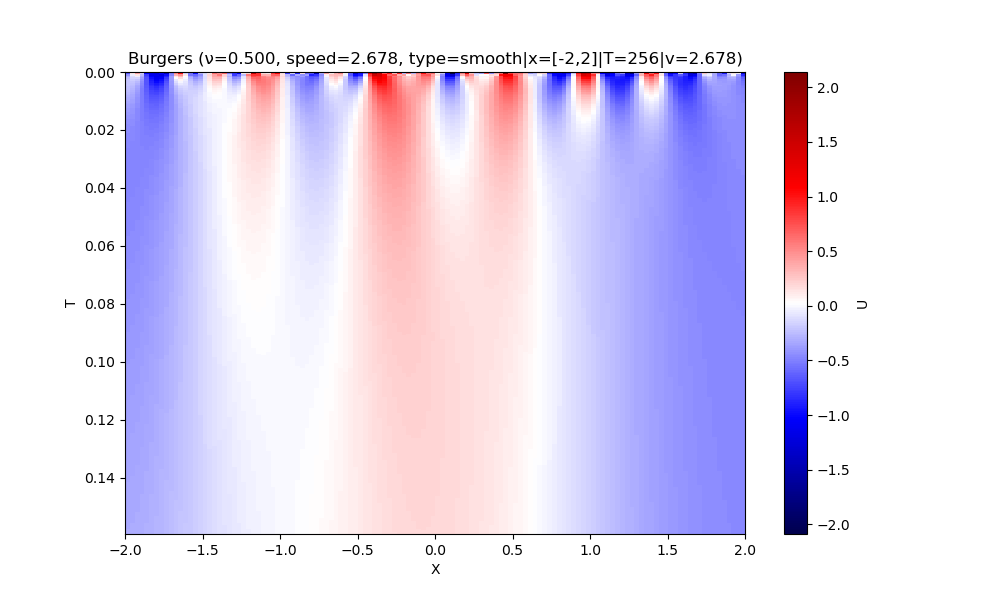
\includegraphics[width=\linewidth]{images/smooth.png}
        \caption{Shock initial condition}
    \end{minipage}
    \hfill
    \begin{minipage}[t]{0.48\textwidth}
        \centering
        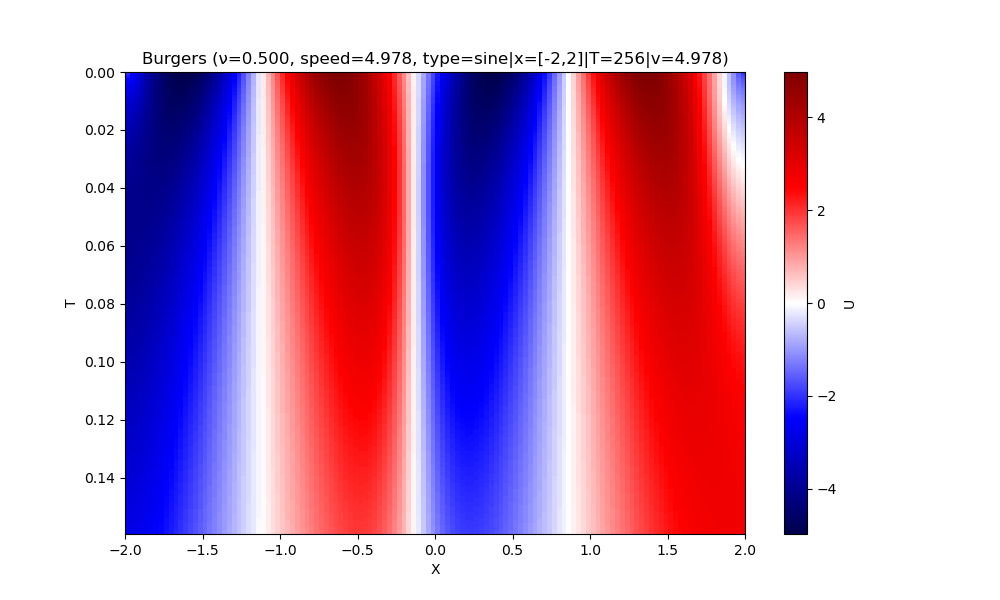
\includegraphics[width=\linewidth]{images/sin.png}
        \caption{Rarefaction initial condition}
    \end{minipage}
    \\[0.5cm]
    \begin{minipage}[t]{0.48\textwidth}
        \centering
        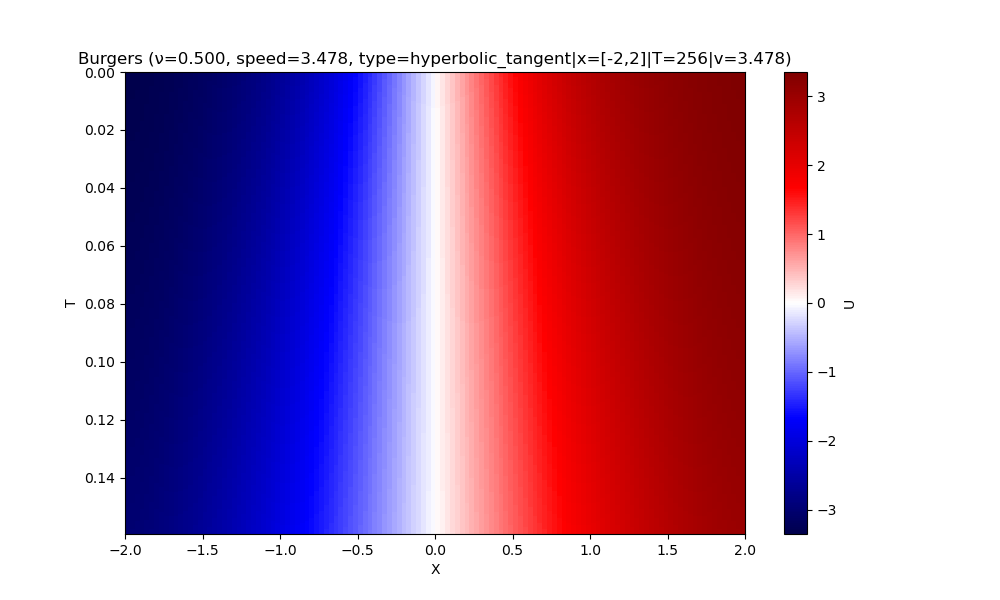
\includegraphics[width=\linewidth]{images/hyperbolic_tangeante.png}
        \caption{Sinusoidal initial condition}
    \end{minipage}
    \hfill
    \begin{minipage}[t]{0.48\textwidth}
        \centering
        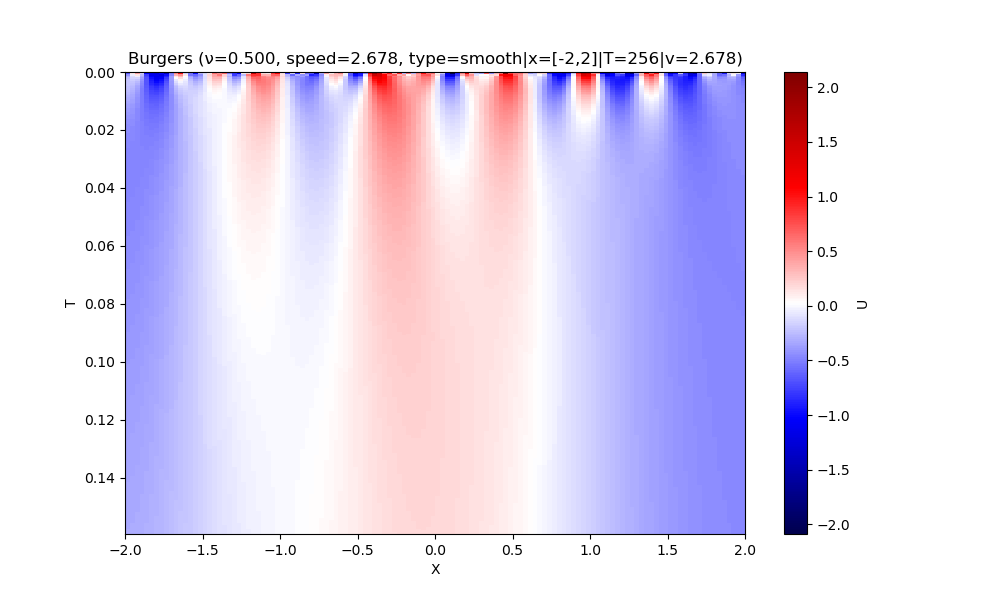
\includegraphics[width=\linewidth]{images/smooth.png}
        \caption{Smoothed random field initial condition}
    \end{minipage}
    \label{fig:initial_conditions}
\end{figure}

\noindent Insert the actual plots produced by the notebook (e.g., \texttt{visualization.py} helpers) in place of the placeholders above.
